\begin{section}{Metodología}
  La creación de un videojuego implica conocimientos muy variados. Los equi- pos de desarrollo suelen ser heterogéneos, y la creatividad juega un papel tan importante, que muchos productores procuran proveer a sus creadores la mayor libertad creativa posible.

  Todos estos factores, sumados, hacen del desarrollo de videojuegos algo pe- culiar. Los ciclos de vida tradicionales, como el waterfall no tienen lugar en su desarrollo (Bates y Bob, 2004), y pese a que las metodologías ágiles parecen encajar bien en este proceso, principalmente el scrum (Chandler y Maxwell, 2009), Paul Miller, un ``veterano'' del desarrollo de videojuegos, critica fuer- temente esta metodología al ser aplicada al desarrollo de videojuegos.(Miller, 2008)

  Pero el desarrollo de videojuegos es solamente una de las etapas para la creación de un videojuego. Aunque existen muchas metodologías para la creación de videojuegos, varios autores(Moore, E, Novak, y Jeannine, 2010)(Bates y Bob, 2004) concuerdan en que todas cuentan con las siguientes etapas:
  \begin{subsection}{Concepción}
    La creación de la idea del videojuego es, en sí, un proceso bastante complica- do. Una jugabilidad cautivante es dificil de crear. Mike Stout, gamedev veterano, publicó la metodología que él usó para la concepción skylanders.

    Aunque existen muchas metodologías, todas ellas están documentadas en li- bros que están detrás de murallas de pago, por esta razón, este proyecto utilizará la metodología trinity.

    \begin{subsubsection}{Trinity}
      Es una metodología de diseño de videojuegos \footnote{Esto es aplicable durante la fase a la que Moore et. al. y Bates denominan: \textit{fase de pre-producción}.} creada por Mike Stout, y, heróicamente compartida en Gamasutra \footnote{Una página que contiene diversos artículos sobre videojuegos, y su desarrollo en general.}

      \paragraph{Principio 1: El juego pregunta, el jugador responde}

      \begin{citation}
        Como diseñador de juegos, tu trabajo (en un sentido muy prácti- co) es hacerle preguntas al jugador. El trabajo de los jugadores es responder a esas preguntas utilizando las herramientas que tú les das.(Stout, 2015)
      \end{citation}

      Este enfoque podría conducir al diseñador a cometer el error de, formular una pregunta, y restringir al jugador únicamente a dos posibles tipos de respuesta: la correcta y la incorrecta, bueno y malo. El planteamiento de este tipo de preguntas no están acorde a esta metodología, ya que obliga al jugador a buscar siempre la respuesta correcta, en vez de que cada pregunta abra un mundo completo de posibilidades con cada una de las posibles respuestas. Debido a que esta dicotomía es muy difícil de evitar, a veces es necesario disfrazarla con el uso de herramientas variadas.

      \paragraph{Preguntas}

      Consiste en una pregunta que ``el juego'' le hace al jugador. Podría no ser obvia para el jugador, pero eventualmente, el jugador debería darse cuenta de lo que el juego le está ``preguntando''.

      El hecho de que el jugador se de cuenta de la pregunta y la rapidez con la que se de cuenta, dependerá de la habilidad del diseñador. El hecho de que el jugador plantee una respuesta correcta, dependerá de la dificultad que el diseñador ponga en el juego.

      \paragraph{Meta preguntas}

      Es una pregunta incompleta que integra el contexto bajo el que se pregunta, pero para ser formulada, debe ser añadida a otra pregunta.

      Las meta preguntas permiten formular preguntas de una forma más específica, y añadir así una jugabilidad variada y entretenida.

      Por ejemplo, si el jugador tiene varias armas, y se encuentra con un enemigo, el enemigo podría formular esta pregunta: ``¿Cómo vas a pasar hacia donde estoy bloqueándote el camino?'', pero más específicamente, la pregunta podría ser: ``¿Cómo vas a derrotarme?'', pero incluso más específia es la pregunta: ``¿Cuál es la forma correcta de atacarme?''. Cada una de estas preguntas incorpora el contexto bajo el que el jugador está jugando, en la primera pregunta, por ejemplo, el enemigo podría estar bloqueando el camino a la salida de alguna cueva que está por derrumbarse. En la segunda, el enemigo podría tener la llave de la puerta de la prisión en la que el protagonista está preso, y en la última, el enemigo podría ser invulnerable a cierto tipo de ataques, o incluso, el jugador podría necesitar un tipo diferente de arma, en función al terreno que rodea al enemigo.

      \paragraph{Respuestas}

      El jugador responde a las preguntas planteadas utilizando las he- rramientas que le han sido dadas. Es importante diseñar estas herramientas, de tal forma, que sean reusables; sobresaturar al jugador con muchas herramien- tas, introduciéndolas todas de golpe, podría llevar a que el jugador se canse de explorarlas y pierda interés. También podría ocurrir que el diseñador pierda control sobre las preguntas que puede plantear, ya que el exceso de posibilidades sin explorar causarán que las preguntas no sean lo suficientemente obvias para el jugador.

      Pero ninguno de los extremos es recomendable. Si las herramieintas que el jugador posee no son lo suficientemente diversas, el juego podría tornarse aburrido, ya que el jugador se vería obligado a seguir una línea que ha sido estréchamente trazada por el diseñador.
    \end{subsubsection}
  \end{subsection}

  \begin{subsection}{Pre-producción}
    También conocida como fase de diseño, durante esta etapa, se diseña el juego, enfocándose en la idea y el concepto. El resultado de esta fase consiste en varios documentos iniciales de diseño, toda esta documentación describirá el itinerario de la implementación del videojuego, el diseño, el concepto, la jugabilidad, la historia y todo lo que define al juego, esta documentación también debería ser fácil de entender y lo menos ambigua posible.

    A continuación, se listan los documentos iniciales resultantes de esta etapa.

    \begin{subsubsection}{High Concept}
      Una descripción corta del juego, hecha con la idea de ``vender'' la idea del juego a un productor, de forma que el juego pueda ser implementado con un buen presupuesto.

      Debe tener de 2 a 3 páginas, y empezar con un párrafo que consista en 2 líneas o menos. El resto de la primera pagina, consiste en una lista de características clave, cada una, descrita en, no más de 3 oraciones. Estas características, deben ser escritas con la idea de describir cómo se verá y sentirá el juego, los detalles de cómo lograr esto no competen a esta sección. Las características más importantes del juego, deben resaltarse en negrilla, de forma que cautiven la atención del lector.

      En la segunda página, va un panorama general, que contiene:

      \begin{itemize}
      \item \textbf{Motivación del jugador} Aquí se describe qué motivación tienen los jugadores para jugarlo.

      \item \textbf{Género}

      \item \textbf{Licensia}

      \item \textbf{Clientes} Aquí se describe qué tipo de persona estaría dispuesta a comprar el juego.

      \item \textbf{Competencia}

      \item \textbf{Hardware} Para qué hardware está hecho el juego?

      \item \textbf{Metas de diseño} Aquí se listan las experiencias que se espera que el juego deje en las personas.
      \end{itemize}


      Y por último, y si es necesario, se puede añadir un poco de información sobre el juego en sí, sobre sus personajes más únicos, o sobre sus mecanismos más alucinantes. Esto, con el objetivo de llamar la atención del lector, y hacer que se enamore del juego.(Adams, 2008)

      Debido a la naturaleza del proyecto, el financiamiento no es una ``pieza clave'', por lo tanto, no se le dará mucha importancia a la realización de este documento.
    \end{subsubsection}

    \begin{subsubsection}{Pitch}
      Es un documento que describe todos los aspectos del juego que pueden ha- cerlo rentable. Todas las estrategias de venta, y lo que se puede hacer para ganar dinero con el videojuego van aquí.

      Debido a la naturaleza del proyecto, el financiamiento no es una ``pieza clave'', por lo tanto, no se le dará mucha importancia a la realización de este documento.
    \end{subsubsection}

    \begin{subsubsection}{Concept}
      Es un documento en el que se describe el juego con más detalle. Es como el hight concept, pero mucho más detallado. Antes de que el juego sea aprobado, programadores y artistas, trabajan juntos para producir este documento.

      Los programadores comienzan a trabajar de forma rápida y un tanto des- preocupada, para generar un prototipo. Los artistas comienzan a desarrollar el concepto de arte, y bosquejos que podrían servir como la piedra inicial de características reales del juego.
    \end{subsubsection}

    \begin{subsubsection}{Game Design Document (GDD)}
      \begin{citation}
        El reto es crear un documento de diseño que le permita a tu proyec- to tolerar adaptaciones inesperadas, sin perder la integridad de su dirección original, ni sus metas.(Freeman, 1997)
      \end{citation}

      Birkhead concuerda en que el documento de diseño debería ser lo suficientemente claro como para que, al finalizar de leerlo, el lector tenga totalmente clara la idea del juego.(Birkhead, 2011)

      El GDD orienta a todos los que están involucrados en el proceso de creación del videojuego, de tal forma que todos tengan muy en claro lo que están haciendo, y aunque es imposible que todos tengan la misma idea, es importante que el márgen de error producido por las indeterminaciones sea mínimo en las características más importantes del juego.

      Tzvi Freeman cree que un buen GDD debe tener estas 10 características clave: (Freeman, 1997)

      \begin{enumerate}
      \item \textbf{Describe el alma del juego} El equipo que crea al videojuego está com- puesto por humanos, creativos, testarudos, fascinantes e impredescibles humanos que aportarán sus ideas y creatividad al juego. Por eso es im- portante describir en este documento, no solo las características del juego, sino que también, la forma en la que debería ``sentirse'' al jugarlo, de esa forma, todos los que están ayudando en hacer al juego realidad, sabrán si sus sugerencias son oportunas o no.
      \item Legible
      \item \textbf{Priorizado} Esto también ayuda a que los integrantes del equipo sepan qué características del juego deben ir sí o sí, y cuáles deben obedecerse al pie de la letra, sin lugar a cambios que tergiversen su sentido. Pero también hay otras características más flexibles, que no necesariamente deben quedar como se escriben en el documento. Estas características tal vez podrían causar una mejora al juego si se cambian por otras ideas.

        Una buena lista de tags podría ser:(Freeman, 1997)

        \begin{itemize}
        \item Indispensable
        \item Importante
        \item Si es posible
        \item Rechazado
        \end{itemize}

      \item \textbf{Detallado} Dentro de más detalles tenga una especificación, más difícil es que se mal entienda. Por eso es importante poner ejemplos, usar una jerga clara, y si ser redundante ayuda a que no hayan ambigüedades, entonces es necesario.

      \item \textbf{Prototipos} Cuando sea necesario Cuando una característica se vuelve muy difícil de entender, a veces es necesario hacer un prototipo para que se entienda. Pero no siempre es buena idea abusar de los prototipos, hay cosas que quedan más claras en palabras.

      \item \textbf{Describe el cómo y el qué (no-técnico)} A veces, la forma en la que se consigue algo, afecta al resultado final. Cuando esto ocurra, es necesario especificar cómo va a lograrse un resultado final. No debe confundirse con detalles técnicos, por ejemplo, con qué algoritmos se va a programar cierto detalle del juego, o con qué herramienta debería dibujarse; aplica únicamente al diseño. Cuando en el GDD se especifique qué es lo que se quiere que el jugador sienta en cierta parte del juego, también debería especificarse exactamente cómo causar que el jugador se sienta de esa forma.

      \item \textbf{Provee alternativas} A veces, cuando una característica requiere muchos recursos, necesita alternativas más baratas. Esto podría implicar mucho tiempo y muchos párrafos dedicados al GDD, si se prioriza correctamente, solo será necesario añadir alternativas a las características indispensables.

      \item \textbf{Tiene vida propia} Debido a que el equipo de desarrollo está compuesto por personas, las personas tienden a ser creativas, y a proponer cambios.

        De hecho, es bastante probable que el creador del juego, y escritor del GDD también aporten nuevos cambios al juego, luego de que el GDD haya sido creado. Por eso es importante que el GDD sea, hasta cieirto punto, flexible. Esta flexibilidad no debe perjudicar a la idea principal del juego, no debe salirse de control, ni cambiar demasiado el rumbo que el juego estaba llevando.

      \item \textbf{Nada ambiguo} Nadie debería poder decir ``lo hice de esa forma porque no estaba en el GDD''. Buena presentación Si trabajas en equipo, y si tu equipo no te conoce, es probable que no lean el GDD si no se ve ``lindo''. Si no se ve lo suficien- temente presentable, podrían creer que no invertiste el suficiente esfuerzo en él, y podría terminar siendo ignorado.
      \end{enumerate}

      Al ser este proyecto un one-man-project, aunque se le dará una gran importancia para definir al juego, y no comenzar a desarrollar a ciegas, no se le dará tanta importancia a desambiguar las características del juego.
    \end{subsubsection}

    \begin{subsubsection}{Prototype}
      Cuando algo no queda lo suficientemente claro en el GDD, realizar prototipos es importante. Pero también es importante prototipar para probar característi- cas experimentales del juego.

      Debido al corto tiempo, y a que el proyecto se llevará a cabo por la crea- dora del juego, el prototipado en la fase de producción no se usará más que en maquetas.
    \end{subsubsection}

  \end{subsection}

  \begin{subsection}{Producción}
    Esta es la etapa principal del desarrollo de un juego, y todo el equipo trabaja de forma concurrente para desarrollar el juego.

    Pese a que Moore y Bates concuerdan en varios pasos que deben seguirse en esta etapa (Moore y cols., 2010) (Bates y Bob, 2004), en este proyecto se utilizará la metodología scrum, con algunos ajustes para que funcione adecua- damente en la producción de videojuegos. Bonin le llama a este tipo de scrum: scrumBut(Bonin, 2014), debido a que es scrum, ``pero'' con modificaciones. Incorporaré algunas de las ideas de Bonin a la metodología que usaré.

    Algunos gamedevs, suelen añadir características de waterfall al scrum, sin embargo, Keith Clinton cree que no es aconsejable aplicar waterfall al desarrollo de un juego, él cree que es mejor añadirle características de lean para solucionar algunos problemas que no pueden ser afrontados correctamente mediante scrum puro.(Keith, 2008) También incorporaré algunas de sus ideas a la metodología.

    Además de estos ajustes, también aplicaré algunos en base a mis experiencias de desarrollo de videojuegos. Esto es necesario porque el equipo de desarrollo consiste en una sola persona, y hay muy poca documentación sobre metodologías de desarrollo de videojuegos para una sola persona.

    \begin{subsubsection}{Causas para crear una nueva metodología}
      No existe una metodología para producir videojuegos mediante un solo gamedev. Los juegos desarrollados por una sola persona suelen tomar más de un año, o ser extremadamente sencillos.

      Muchos de los juegos creados por un solo gamedev son abandonados, por lo que este proyecto ya tiene una alta probabilidad de fracasar.

      Es imposible usar una metodología ya existente, debido a que todas estas me- todologías han sido creadas y ajustadas por gamedevs expertos, y ellos trabajan en proyectos grandes, en grandes compañías con grandes y multidisciplinarios equipos. Ellos no tienen que preocuparse de que el desarrollador no quiera pro- gramar, porque tiene un ataque de creatividad y prefiere dibujar un sprite. Ellos se preocupan porque todos los miembros se mantengan en sus roles y terminen el trabajo que se les ha asignado.

      Si algún miembro tiene un ataque de creatividad, y quiere realizar una tarea que no debería desempeñar, tendrá que esperar a que el trabajo que se le ha asignado esté terminado, o a su tiempo libre, porque, después de todo, es muy poco probable que su idea sea mejor que la de un profesional en esa área.

      Cuando un gamedev trabaja solo, debe aprovechar al máximo esos ataques de creatividad, pero, si tiene un límite de tiempo y presupuesto, no debe invertir más tiempo del ``necesario'', debe medir su tiempo y esfuerzo de acuerdo a la curva de satisfacción del jugador vs costo.

      A esta metodología yo le llamo lone-ranger-methodology, o en español: me- todología del llanero solitario, ya que se aprovechan las mejores características de metodologías ágiles como lean y scrum, y las adapta a un trabajo en el que un solo gamedev hace todo el trabajo.

    \end{subsubsection}

    \begin{subsubsection}{La metodología del Llanero Solitario}
      Es una metodología de desarrollo de videojuegos, que aprovecha las mejores características de metodologías ágiles como lean y scrum, y las adapta al desarrollo de videojuegos llevado a cabo por un solo \textit{gamedev}

      \paragraph{Ciclo de vida}

      \begin{center}
        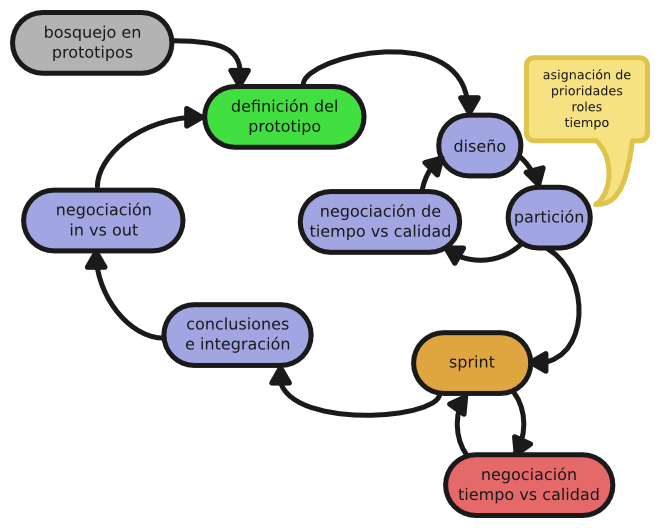
\includegraphics[width=.9\textwidth]{lifecycle.png}
      \end{center}

      \paragraph{Bosquejo en prototipos} Se define un plan de prototipos. El objetivo es tener un panorama general de la forma en la que el prototipado nos llevará a finalizar el juego. Este plan no debe ser demasiado detallado.

      \paragraph{Definición del prototipo} Se define a pleno detalle el prototipo que se espera tener funcionando al finalizar el ciclo. Es importante que los prototipos no sean ambiciosos, el flujo de entrega de los prototipos debe permanecer constante.

      \paragraph{Diseño} Se diseña, a grandes razgos el código del prototipo, y se describe el trabajo que se tiene que hacer mediante modelos. La idea de esta fase, es que el llanero solitario tenga una vaga idea de cómo va a hacer el prototipo.

      \paragraph{Partición} El modelo se parte en pequeñas particiones. Cada partición tiene asignado un rol, una prioridad dentro de una escala del 1 al 10, y por último, se calcula el tiempo estimado que cada partición tomará en finalizarse.

      \paragraph{Negociación de tiempo vs calidad} En base al tiempo que tomará el sprint en finalizarse, se revisan las particiones. Si el tiempo es demasiado grande, se deben negociar características, sacrificando calidad para que el tiempo de reali- zación sea más corto. Si existieron negociaciones, se revisa el diseño y se parti- cionan las partes afectadas de nuevo.

      \paragraph{Sprint} Se implementa cada una de las particiones hechas en la fase anterior.

      El orden tiene muy poca importancia, el llanero solitario puede elegir las particiones en base a lo que le parezca más divertido hacer, también puede cambiar de tarea, si de pronto quiere trabajar en otra cosa.

      Es importante que tenga en cuenta que las tareas marcadas con una prioridad baja, deben finalizarse lo más rápido posible, de tal forma que, si surje algún inconveniente en las tareas con prioridades altas, pueda ser compensado con el tiempo sobrante de las tareas con prioridad baja.

      Cuando el llanero solitario finaliza una de las particiones, debe anotar el saldo de tiempo con el que la terminó.

      \paragraph{Negociación tiempo vs calidad} Si el llanero solitario siente que está invir- tiendo demasiado tiempo en una partición, debería negociar tiempo vs calidad para completar la característica. Si el tiempo que está invirtiendo en esa par- tición excede del 125 \% del tiempo destinado, deberá abandonarla y terminar todas las particiones que no dependan imprescindiblemente de esa partición.

      \paragraph{Conclusiones e integración} Si el prototipo construido no está integrado al resto de prototipos, se integra en esta fase. También se documenta y limpia el código, y se pone en su sitio todos los assets que podrían estar fuera de su lugar.

      Se realiza una lista de las particiones que no se pudieron finalizar, y las causas por las que no se pudo hacer descritas brevemente, esto se documenta en la lista de undone. También se realiza una lista de las nuevas ideas que hayan surgido, y de las características inconclusas de las particiones. Las ideas se documentan en la lista de ideas, y las características inconclusas, en la lista de good to have.

      \paragraph{Negociación in vs out} Si existen particiones sin finalizar en la lista de undo- ne, cada una de las particiones deberá ser negociada. El llanero solitario debe determinar qué tan importante es esa partición, y si vale la pena ponerla de nuevo en el siguiente prototipo. Esto se determina en base al tiempo y esfuerzo que tomaría finalizar la partición, y a la importancia de finalizarla.
    \end{subsubsection}
  \end{subsection}
\end{section}
